% Options for packages loaded elsewhere
\PassOptionsToPackage{unicode}{hyperref}
\PassOptionsToPackage{hyphens}{url}
%
\documentclass[
]{article}
\usepackage{amsmath,amssymb}
\usepackage{iftex}
\ifPDFTeX
  \usepackage[T1]{fontenc}
  \usepackage[utf8]{inputenc}
  \usepackage{textcomp} % provide euro and other symbols
\else % if luatex or xetex
  \usepackage{unicode-math} % this also loads fontspec
  \defaultfontfeatures{Scale=MatchLowercase}
  \defaultfontfeatures[\rmfamily]{Ligatures=TeX,Scale=1}
\fi
\usepackage{lmodern}
\ifPDFTeX\else
  % xetex/luatex font selection
\fi
% Use upquote if available, for straight quotes in verbatim environments
\IfFileExists{upquote.sty}{\usepackage{upquote}}{}
\IfFileExists{microtype.sty}{% use microtype if available
  \usepackage[]{microtype}
  \UseMicrotypeSet[protrusion]{basicmath} % disable protrusion for tt fonts
}{}
\makeatletter
\@ifundefined{KOMAClassName}{% if non-KOMA class
  \IfFileExists{parskip.sty}{%
    \usepackage{parskip}
  }{% else
    \setlength{\parindent}{0pt}
    \setlength{\parskip}{6pt plus 2pt minus 1pt}}
}{% if KOMA class
  \KOMAoptions{parskip=half}}
\makeatother
\usepackage{xcolor}
\usepackage[margin=1in]{geometry}
\usepackage{color}
\usepackage{fancyvrb}
\newcommand{\VerbBar}{|}
\newcommand{\VERB}{\Verb[commandchars=\\\{\}]}
\DefineVerbatimEnvironment{Highlighting}{Verbatim}{commandchars=\\\{\}}
% Add ',fontsize=\small' for more characters per line
\usepackage{framed}
\definecolor{shadecolor}{RGB}{248,248,248}
\newenvironment{Shaded}{\begin{snugshade}}{\end{snugshade}}
\newcommand{\AlertTok}[1]{\textcolor[rgb]{0.94,0.16,0.16}{#1}}
\newcommand{\AnnotationTok}[1]{\textcolor[rgb]{0.56,0.35,0.01}{\textbf{\textit{#1}}}}
\newcommand{\AttributeTok}[1]{\textcolor[rgb]{0.13,0.29,0.53}{#1}}
\newcommand{\BaseNTok}[1]{\textcolor[rgb]{0.00,0.00,0.81}{#1}}
\newcommand{\BuiltInTok}[1]{#1}
\newcommand{\CharTok}[1]{\textcolor[rgb]{0.31,0.60,0.02}{#1}}
\newcommand{\CommentTok}[1]{\textcolor[rgb]{0.56,0.35,0.01}{\textit{#1}}}
\newcommand{\CommentVarTok}[1]{\textcolor[rgb]{0.56,0.35,0.01}{\textbf{\textit{#1}}}}
\newcommand{\ConstantTok}[1]{\textcolor[rgb]{0.56,0.35,0.01}{#1}}
\newcommand{\ControlFlowTok}[1]{\textcolor[rgb]{0.13,0.29,0.53}{\textbf{#1}}}
\newcommand{\DataTypeTok}[1]{\textcolor[rgb]{0.13,0.29,0.53}{#1}}
\newcommand{\DecValTok}[1]{\textcolor[rgb]{0.00,0.00,0.81}{#1}}
\newcommand{\DocumentationTok}[1]{\textcolor[rgb]{0.56,0.35,0.01}{\textbf{\textit{#1}}}}
\newcommand{\ErrorTok}[1]{\textcolor[rgb]{0.64,0.00,0.00}{\textbf{#1}}}
\newcommand{\ExtensionTok}[1]{#1}
\newcommand{\FloatTok}[1]{\textcolor[rgb]{0.00,0.00,0.81}{#1}}
\newcommand{\FunctionTok}[1]{\textcolor[rgb]{0.13,0.29,0.53}{\textbf{#1}}}
\newcommand{\ImportTok}[1]{#1}
\newcommand{\InformationTok}[1]{\textcolor[rgb]{0.56,0.35,0.01}{\textbf{\textit{#1}}}}
\newcommand{\KeywordTok}[1]{\textcolor[rgb]{0.13,0.29,0.53}{\textbf{#1}}}
\newcommand{\NormalTok}[1]{#1}
\newcommand{\OperatorTok}[1]{\textcolor[rgb]{0.81,0.36,0.00}{\textbf{#1}}}
\newcommand{\OtherTok}[1]{\textcolor[rgb]{0.56,0.35,0.01}{#1}}
\newcommand{\PreprocessorTok}[1]{\textcolor[rgb]{0.56,0.35,0.01}{\textit{#1}}}
\newcommand{\RegionMarkerTok}[1]{#1}
\newcommand{\SpecialCharTok}[1]{\textcolor[rgb]{0.81,0.36,0.00}{\textbf{#1}}}
\newcommand{\SpecialStringTok}[1]{\textcolor[rgb]{0.31,0.60,0.02}{#1}}
\newcommand{\StringTok}[1]{\textcolor[rgb]{0.31,0.60,0.02}{#1}}
\newcommand{\VariableTok}[1]{\textcolor[rgb]{0.00,0.00,0.00}{#1}}
\newcommand{\VerbatimStringTok}[1]{\textcolor[rgb]{0.31,0.60,0.02}{#1}}
\newcommand{\WarningTok}[1]{\textcolor[rgb]{0.56,0.35,0.01}{\textbf{\textit{#1}}}}
\usepackage{graphicx}
\makeatletter
\def\maxwidth{\ifdim\Gin@nat@width>\linewidth\linewidth\else\Gin@nat@width\fi}
\def\maxheight{\ifdim\Gin@nat@height>\textheight\textheight\else\Gin@nat@height\fi}
\makeatother
% Scale images if necessary, so that they will not overflow the page
% margins by default, and it is still possible to overwrite the defaults
% using explicit options in \includegraphics[width, height, ...]{}
\setkeys{Gin}{width=\maxwidth,height=\maxheight,keepaspectratio}
% Set default figure placement to htbp
\makeatletter
\def\fps@figure{htbp}
\makeatother
\setlength{\emergencystretch}{3em} % prevent overfull lines
\providecommand{\tightlist}{%
  \setlength{\itemsep}{0pt}\setlength{\parskip}{0pt}}
\setcounter{secnumdepth}{5}
\ifLuaTeX
  \usepackage{selnolig}  % disable illegal ligatures
\fi
\usepackage[]{biblatex}
\addbibresource{biblio.bib}
\usepackage{bookmark}
\IfFileExists{xurl.sty}{\usepackage{xurl}}{} % add URL line breaks if available
\urlstyle{same}
\hypersetup{
  pdftitle={Projet Poisson: Modèle de réparation imparfaite de Brown-Proschan},
  pdfauthor={Arman Hosseini, Paul Slisse, Guillaume Staub, Jade Roumazeille-Peter},
  hidelinks,
  pdfcreator={LaTeX via pandoc}}

\title{Projet Poisson: Modèle de réparation imparfaite de
Brown-Proschan}
\author{Arman Hosseini, Paul Slisse, Guillaume Staub, Jade
Roumazeille-Peter}
\date{2025-03-14}

\begin{document}
\maketitle

{
\setcounter{tocdepth}{2}
\tableofcontents
}
\newpage

\section{Présentation du modèle}\label{pruxe9sentation-du-moduxe8le}

\subsection{Introduction}\label{introduction}

Dans ce projet, nous allons nous intéresser au processus de Poisson à
réparation imparfaite dévellopé par Brown et Proschan
\autocite{Brown1983} en 1983 ,retravaillé par Whitaker et Samaniego
\autocite{Whitaker1989},que nous allons raccourcir en BP. Dans ce
modèle, lorsque le système tombe en panne, celui-ci est réparé
``parfaitement'' avec une probabilité \(p\): il redevient donc dans un
état neuf. Sinon, le système est remis dans un état équivalent à celui
précédant la panne.

Pour ce faire, commençons par introduire les notations qui nous seront
nécessaires. On note \(T_i\) les temps entre chaque panne. On note
\(A_i\) l'âge du système après la \(i\)-ème panne. Ainsi, \(A_i=0\) si
l'on a une réparation parfaite après la \(i\)-ème panne et
\(A_i=A_{i-1}+T_i>0\) sinon. On note \(F\) la fonction de répartition de
l'âge sur \([0,+\infty]\) et \(S\) la fonction de survie associé à \(F\)
notée \(S(t)=P(T>t)=1-F(t)\).

Ainsi, les paramètres à estimer de notre modèle sont \((p,F)\).

\subsection{\texorpdfstring{Estimation des paramètres
\((p,F)\)}{Estimation des paramètres (p,F)}}\label{estimation-des-paramuxe8tres-pf}

Pour le modèle de BP, les paramètres \((p,F)\) ne peuvent pas être
estimés avec la seule connaissance de la distribution des \(T_i\). En
effet, on peut montrer que pour deux valeurs de \(p\) différentes et la
même fonction \(F\), il est possible d'obtenir la même distribution des
\(T_i\). Par exemple, si \(F\) est la fonction de répartition d'une loi
exponentielle, alors les \(T_i\) suivent la même loi exponentielle qui
est indépendante de \(p\). Bien que la fonction \(F\) peut être estimée
via les \(T_i\), le problème est que l'on ne peut estimer le paramètre
\(p\) avec la suite des \(T_i\).

Pour remédier à cela, nous allons introduire une nouvelle suite de
variables aléatoires de Bernoulli de paramètre \(p\) que l'on note
\(Z_i\). A la \(i\)-ème panne, si la réparation est parfaite alors
\(Z_i=1\) et si elle est imparfaite, \(Z_i=0\). Rajouter cette
information sur le type de panne qui est uniquement determiné par le
paramètre \(p\) rend le problème d'estimation solvable.

A partir de maintenant, nous allons faire les hypothèses suivantes pour
notre étude : -\(p>0\) -\(F\) est absolument continue (admet une densité
\(f\)) -\(F(0)=0\) (pas de réparation instantanée)

Nous allons observer le système jusqu'à la \(m\)-ème réparation
parfaite. On note \(n\) le nombre total de panne et donc \(n-m\) est le
nombre de réparation imparfaite.

La suite des âges observés \((a_i)\) est entièrement déterminé par les
couples \((t_i,z_i)\). \[
L(p,F)=f(t_1)p^{z_1}(1-p)^{1-z_1}\times\frac{f(t_2+a_1)}{S(a_1)}p^{z_2}(1-p)^{1-z_2}\times ...\times\frac{f(t_n+a_{n-1})}{S(a_{n-1})}p^{z_n}(1-p)^{1-z_n}
\] Pour comprendre cette formulation de la vraisemblance, on considère
le cas n = 2 (les n \textgreater{} 2 se comprennent par récurrence).

\[
L(p,F|(t_1,t_2),(z_1, z_2))=f_{T_1,Z_1}(t_1, z_1)f_{T_2,Z_2}((t_2, z_2)|(T_1 = t_1, Z_1 = z_1))
\]

Par indépendance des événements ``panne'' est ``la réparation est
parfaite'', on a :

\[
f_{T_1,Z_1}(t_1, z_1) = f(t_1)p^{z_1}(1-p)^{1-z_1}
\] Ensuite, on a deux cas possibles :

Si \(z_1 = 0\) (réparation imparfaite), on a \(a_1 = t_1\) :

\[
f_{T_2,Z_2}((t_2, z_2)|(T_1 = t_1, Z_1 = z_1)) = \frac{f(t_2+a_1)}{S(a_1)} p^{z_2} (1-p)^{1-z_2}
\]

Si \(z_1 = 1\) (réparation imparfaite), on a \(a_1 = 0\) et
\(S(a_1) = 1\), d'où :

\[
f_{T_2,Z_2}((t_2, z_2)|(T_1 = t_1, Z_1 = z_1)) = f(t_2) p^{z_2} (1-p)^{1-z_2} = \frac{f(t_2+a_1)}{S(a_1)} p^{z_2} (1-p)^{1-z_2}
\] En notant \(x_i\) l'âge observé juste avant la \(i\)-ème panne. Si
\(z_i=0\), on a directement que \(a_i=x_i\), si \(z_i=1\), \(a_i=0\),
\(x_i=a_{i-1} +t_i\), mais on peut tout de même écrire que
\(S(a_i)=S(x_i)^{1-z_i}\). Si dans la formule de la vraisemblance, on
remplace les \(a_i\) par les \(x_i\) et qu'on factorise les \(p\) et
\((1-p)\) ensemble à l'aide des \(n\) et \(m\) on obtient:

\[
L(p,F)=p^{m}(1-p)^{n-m}f(x_1) \frac{f(x_2)}{S(x_1)^{1-z_1}}\times ...\times\frac{f(x_n)}{S(x_{n-1})^{1-z_{n-1}}}
\]

Avec cette écriture de la vraisemblance, on trouve le MLE de \(p\):
\(\hat p =\frac{m}{n}\). Ce résultat est plutôt logique, on estime la
probabilité \(p\) de réparation parfaite en calculant le ratio de
réparation parfaite sur le nombre total de pannes.

Maintenant qu'on a le MLE de \(p\), intéressons nous à \(F\).

Pour trouver un estimateur empirique du MLE de F, on peut maximiser la
partie ne dépendant pas de \(p\) dans la vraisemblance au dessus. Cela
équivaut à déterminer \(F\), qui est une fonction continue par morceaux,
maximisant, l'estimation suivante de la vraisemblance: \[
l(F)= \prod^n_{i=1}\frac{(F(x_{(i)})-F(x_{(i)}^-))}{S(x_{(i-1)})^{1-z_{(i-1)}}}
\] où la densité \(f\) en \(x_i\) est approximée par
\(F(x_{(i)})-F(x_{(i)}^-)\),les \(x_{(i)}\) sont les âges \(x_i\) avant
les pannes ordonnés. Les \(z_{(i)}\) ne sont pas ordonnés mais sont les
\(z_i\) réindexés pour que \(z_{(i)}\) correspondent au mode de
réparation après la panne survenue à l'âge \(x_{(i)}\). En particulier
notre MLE empirique ne sera pas nécessairement continue à l'inverse de
la vraie fonction \(F\).

Malheureusement, le maximum de la fonction \(l(F)\) n'est pas toujours
atteignable. En effet, il faut que \(z_{(n-1)} = 1\).

Plaçons nous dans le cas où \(z_{(n-1)}=1\). Définissons
\(\phi_i=\frac{S(x_{(i)})}{S(x_{(i-1)})}\) la probabilité de survivre
jusqu'à l'âge \(x_{(i)}\) sachant que le système n'a pas eu de
réparation parfaite depuis une durée \(x_{(i-1)}\). Ainsi, notre
problème de maximisation revient à maximiser par rapport à \(\phi\): \[
l(\phi)=\prod^n_{i=1}(1-\phi_i)\phi_i^{k_i}
\] où \(k_i=\sum^{n-1}_{j=i} z_{(j)}\) est le nombre de réparation
parfaites pour des pannes intervenues à un âge supérieur à \(x_{(i)}\).

On montre facilement que le maximum de cette fonction est atteint en :
\[
\hat\phi_i=\frac{k_i}{k_i+1} , 1\leq i\leq n-1 ; \hat\phi_n=0 
\] Ainsi, on obtient le MLE empirique de la fonction de survie \(S\): \[
\hat{S}(t) =
\left\{
\begin{array}{ll}
  1, & t < x_{(1)} \\
  \prod\limits_{j=1}^{i} \hat{\phi}_j, & x_{(i)} < t < x_{(i+1)}, \quad i=1,\dots,n-1 \\
  0, & t \geq x_{(n)}
\end{array}
\right.
\]

Dans le cas où \(z_{(n-1)}=0\), on a toujours le même maximiseur de
\(l(\phi)\) mais désormais par définition, \(k_{n-1}=0\) et donc
\(\hat\phi_{n-1}=0\) ce qui implique que
\(\hat S(t)=0, t \geq x_{(n-1)}\). Ainsi, on voit que notre
approximation de la vraisemblance \(l(F)\) n'est pas défini car dans le
dernier terme du produit, on a une division par 0. C'est pourquoi dans
ce cas précis, il n'existe pas de MLE empirique issu de la maximisation
de notre estimation de la vraisemblance. Ce MLE empirique est en réalité
un ``neighbourhood MLE'' de F dans une certaine topologie, on peut tout
de même l'utiliser pour \(z_{(n-1)}=0\).

Ce modèle de BP peut-être vu comme une suite de réparations parfaites
indépendantes, ainsi, on peut se restreindre aux temps de réparations
parfaites pour étudier les propriétés du modèle. On a le résultat
suivant (citer BP 1983) qui nous dit que si \(Y_1\) est l'âge du système
à la première réparation parfaite, alors la fonction de survie \(S_y\)
de \(Y_1\) vérifie: \[
S_y(t)=(S(t))^p
\]

En effet, en notant \(r\) le taux de hasard associé à \(T\), le taux de
hasard associé à \(Y_1\) est égal à \(pr\) car la probabilité qu'une
réparation ait lieu à l'instant t sachant qu'il n'y avait pas
précédemment est égale à \(r(t)\), et elle est alors parfaite avec une
probabilité \(p\), avec indépendance entre les deux phénomènes. On peut
ensuite utiliser le lien entre taux de hasard et fonction de survie: \[
S_y(t)=exp(-\int_0^t p r(x) dx)=(S(t))^p
\] En établissant la distribution empirique du processus de Poisson
inhomogène obtenu en ne considérant que les durées entre deux
réparations parfaites \(Y_1\), \ldots{} , \(Y_m\). On obtient ainsi une
approximation de \(S_y\), que l'on note \(\hat S_y\). Or
\(S_y(t)=(S(t))^p\), donc on obtient via \(1 - \hat S_y ^{n/m}\) un
autre estimateur de la fonction de répartition.

On peut également établir la distribution empirique des
\(T_i | Z_{i-1} = 1\), c'est-à-dire des durées entre chaque réparation
parfaite et la réparation suivante. On obtient ainsi une approximation
de la densité, et en la cumulant, une nouvelle estimation de la fonction
de répartition.

Ces deux derniers estimateurs n'exploitent pas toutes les informations
issues des observations de \(T\) et \(Z\), contrairement au premier, on
peut donc supposer qu'ils seront moins performants.

\section{Modelisation numerique}\label{modelisation-numerique}

\subsection{Simulation d'un processus de
Weibull}\label{simulation-dun-processus-de-weibull}

Les \(Z_i\) suivent une loi Binomiale par leur définition:
\(\mathbb{P}(Z_i=1)=p\).

On simule ici le modèle. Pour ce faire, on commence par créer deux
fonctions: \(simulPPh1\) et \(invWeibull\). La fonction \(simulPPh1\)
permet de simuler un processus de poisson homogène: on simule \(k\) fois
une variable aléatoire suivant la loi exponentielle de paramètre 1 ce
qui nous donne une liste de nombres telle que \([n_1 , n_2,...,n_k]\).
On renvoie ensuite les temps d'arrivés simulés (notés \(A_k\) dans la
fonction \(simulPPIWeibull\) ) qui représentent la somme cumulée telle
que \([n_1, n_1+n_2,... , n_1+...+n_k]\).

\begin{Shaded}
\begin{Highlighting}[]
\NormalTok{simulPPh1 }\OtherTok{\textless{}{-}} \ControlFlowTok{function}\NormalTok{(k)}
\NormalTok{\{}
  \FunctionTok{return}\NormalTok{(}\FunctionTok{cumsum}\NormalTok{(}\FunctionTok{rexp}\NormalTok{(k, }\DecValTok{1}\NormalTok{)))}
\NormalTok{\}}
\end{Highlighting}
\end{Shaded}

La fonction \(invWeibull\) renvoie l'intensité cumulée inverse de
Weibull: \(\Lambda^{-1}\). Montrons comment nous l'avons trouvé:

Nous avons prouvé en cours que la fonction d'intensité cumulée est égale
à \(\Lambda(t)=(\frac{t}{\alpha})^{\beta}\) avec \(\alpha , \beta\) des
paramètres strictement positifs. Calculons l'inverse de cette fonction:
\[
y=(\frac{t}{\alpha})^{\beta}
\iff
y^{\frac{1}{\beta}} = \frac{t}{\alpha}
\iff
t=\alpha y^{\frac{1}{\beta}}
\] Ainsi, \(\Lambda^{-1}(y)=\alpha y^{\frac{1}{\beta}}\). On
l'implémente donc avec comme paramètres par défaut \(\beta=2\) et
\(\alpha=1\).

\begin{Shaded}
\begin{Highlighting}[]
\NormalTok{invWeibull }\OtherTok{\textless{}{-}} \ControlFlowTok{function}\NormalTok{(y, }\AttributeTok{alpha=}\DecValTok{1}\NormalTok{, }\AttributeTok{beta=}\DecValTok{2}\NormalTok{)}
\NormalTok{\{}
  \FunctionTok{return}\NormalTok{(alpha}\SpecialCharTok{*}\NormalTok{y}\SpecialCharTok{**}\NormalTok{(}\DecValTok{1}\SpecialCharTok{/}\NormalTok{beta))}
\NormalTok{\}}
\end{Highlighting}
\end{Shaded}

On peut maintenant simuler le modèle BP. Pour cela, on génère une
variable aléatoire géométrique de paramètre \(p\), représentant le
nombre \(k\) de réparations imparfaites nécessaires avant d'atteindre la
première réparation parfaite. On simule ensuite le processus homogène
comme expliqué précédemment et on retourne les temps
\(T_i = \Lambda^{-1}(A_i)\) et les valeurs de la fonction de survie de
la loi Weibull: \(S(t)=exp{(-(\frac{t}{\alpha})^{\beta})}\) créant ainsi
un processus de poisson inhomogène. On réitère cela \(m\) fois où \(m\)
représente le nombre de réparations parfaites.

\subsection{Première simulation d'un processus de
Brown-Proschan}\label{premiuxe8re-simulation-dun-processus-de-brown-proschan}

\begin{Shaded}
\begin{Highlighting}[]
\NormalTok{simulPPIWeibull }\OtherTok{\textless{}{-}} \ControlFlowTok{function}\NormalTok{(m, alpha, beta, p)}
\NormalTok{\{}
\NormalTok{  k }\OtherTok{\textless{}{-}} \FunctionTok{rgeom}\NormalTok{(}\DecValTok{1}\NormalTok{, p)}\SpecialCharTok{+}\DecValTok{1}
\NormalTok{  A\_k }\OtherTok{=} \FunctionTok{simulPPh1}\NormalTok{(k)}
\NormalTok{  T\_k }\OtherTok{=} \FunctionTok{c}\NormalTok{(}\FunctionTok{invWeibull}\NormalTok{(A\_k, alpha, beta))}
\NormalTok{  S\_k }\OtherTok{=} \FunctionTok{c}\NormalTok{(}\FunctionTok{exp}\NormalTok{(}\SpecialCharTok{{-}}\NormalTok{(}\FunctionTok{head}\NormalTok{(T\_k,}\SpecialCharTok{{-}}\DecValTok{1}\NormalTok{)}\SpecialCharTok{/}\NormalTok{alpha)}\SpecialCharTok{**}\NormalTok{beta),}\DecValTok{1}\NormalTok{) }
\NormalTok{  T\_succes }\OtherTok{=} \FunctionTok{c}\NormalTok{(}\FunctionTok{tail}\NormalTok{(T\_k,}\DecValTok{1}\NormalTok{)) }\CommentTok{\#le temps où il ya la rep parfaite}
\NormalTok{  S\_succes }\OtherTok{=} \FunctionTok{c}\NormalTok{(}\FunctionTok{tail}\NormalTok{(S\_k,}\DecValTok{1}\NormalTok{)) }\CommentTok{\#et sa valeur de fonction de survie associée}
  \ControlFlowTok{for}\NormalTok{(i }\ControlFlowTok{in} \DecValTok{1}\SpecialCharTok{:}\NormalTok{m}\DecValTok{{-}1}\NormalTok{)}
\NormalTok{  \{}
\NormalTok{   k }\OtherTok{\textless{}{-}} \FunctionTok{rgeom}\NormalTok{(}\DecValTok{1}\NormalTok{, p)}\SpecialCharTok{+}\DecValTok{1}
\NormalTok{   A\_k }\OtherTok{=} \FunctionTok{simulPPh1}\NormalTok{(k)}
\NormalTok{   T\_k\_temp }\OtherTok{=} \FunctionTok{c}\NormalTok{(}\FunctionTok{invWeibull}\NormalTok{(A\_k, alpha, beta))}
\NormalTok{   T\_k }\OtherTok{=} \FunctionTok{c}\NormalTok{(T\_k, }\FunctionTok{tail}\NormalTok{(T\_k,}\DecValTok{1}\NormalTok{) }\SpecialCharTok{+}\NormalTok{ T\_k\_temp)}
\NormalTok{   S\_k }\OtherTok{=} \FunctionTok{c}\NormalTok{(S\_k,}\FunctionTok{exp}\NormalTok{(}\SpecialCharTok{{-}}\NormalTok{(T\_k\_temp[}\SpecialCharTok{{-}}\DecValTok{1}\NormalTok{]}\SpecialCharTok{/}\NormalTok{alpha)}\SpecialCharTok{**}\NormalTok{beta),}\DecValTok{1}\NormalTok{)}
\NormalTok{   T\_succes }\OtherTok{=} \FunctionTok{c}\NormalTok{(T\_succes, }\FunctionTok{tail}\NormalTok{(T\_k,}\DecValTok{1}\NormalTok{))}
\NormalTok{   S\_succes }\OtherTok{=} \FunctionTok{c}\NormalTok{(S\_succes, }\FunctionTok{tail}\NormalTok{(S\_k,}\DecValTok{1}\NormalTok{))}
\NormalTok{  \}}
  \FunctionTok{return}\NormalTok{(}\FunctionTok{list}\NormalTok{(}\AttributeTok{T =}\NormalTok{ T\_k,}\AttributeTok{S=}\NormalTok{S\_k, }\AttributeTok{T\_succes =}\NormalTok{ T\_succes,}\AttributeTok{S\_succes=}\NormalTok{S\_succes))}
\NormalTok{\}}
\end{Highlighting}
\end{Shaded}

On va désormais afficher les résultats d'une simulation de notre
processus de BP pour vérifier que notre code marche bien. Pour cela, on
affiche pour chaque temps de pannes, la valeur de la fonction de survie
théorique (calculable explicitement dans le cas de Weibull).

\begin{Shaded}
\begin{Highlighting}[]
\NormalTok{m }\OtherTok{\textless{}{-}} \DecValTok{5}
\NormalTok{p }\OtherTok{\textless{}{-}} \FloatTok{0.2}
\NormalTok{result }\OtherTok{\textless{}{-}} \FunctionTok{simulPPIWeibull}\NormalTok{(m, }\DecValTok{4}\NormalTok{, }\DecValTok{2}\NormalTok{, p)}
\FunctionTok{print}\NormalTok{(result)}
\end{Highlighting}
\end{Shaded}

\begin{verbatim}
## $T
##  [1]  4.753578  5.595522  7.529124  7.555395 10.373910 11.842220 13.780466
##  [8] 14.647076 15.951219 17.329188 19.268395 19.673077 19.828269 24.823941
## [15] 25.443111 27.180252 27.586065 28.850479 31.270569 31.505093 38.640594
## [22] 39.039584 39.177658 39.836986 40.911724 42.915640 45.606652 48.739325
## [29] 49.260987 50.108287
## 
## $S
##  [1] 2.435868e-01 1.413004e-01 2.892695e-02 1.000000e+00 3.170948e-01
##  [6] 8.874668e-02 4.314252e-02 1.220858e-02 2.553118e-03 1.888327e-04
## [11] 1.033500e-04 8.157684e-05 1.000000e+00 1.394007e-01 3.410782e-02
## [16] 2.324970e-02 6.173325e-03 2.793933e-04 1.990880e-04 1.000000e+00
## [21] 2.878114e-02 2.524149e-02 1.305247e-02 3.964822e-03 1.000000e+00
## [26] 2.521713e-01 2.172136e-02 1.281822e-02 1.000000e+00 1.000000e+00
## 
## $T_succes
## [1]  7.555395 19.828269 31.505093 40.911724 49.260987 50.108287
## 
## $S_succes
## [1] 1 1 1 1 1 1
\end{verbatim}

\begin{Shaded}
\begin{Highlighting}[]
\NormalTok{df\_result }\OtherTok{\textless{}{-}} \FunctionTok{data.frame}\NormalTok{(}\AttributeTok{T =}\NormalTok{ result}\SpecialCharTok{$}\NormalTok{T, }\AttributeTok{S =}\NormalTok{ result}\SpecialCharTok{$}\NormalTok{S)}
\NormalTok{df\_succes }\OtherTok{\textless{}{-}} \FunctionTok{data.frame}\NormalTok{(}\AttributeTok{T =}\NormalTok{ result}\SpecialCharTok{$}\NormalTok{T\_succes, }\AttributeTok{S =}\NormalTok{ result}\SpecialCharTok{$}\NormalTok{S\_succes)}

\FunctionTok{ggplot}\NormalTok{(df\_result, }\FunctionTok{aes}\NormalTok{(}\AttributeTok{x =}\NormalTok{ T, }\AttributeTok{y =}\NormalTok{ S)) }\SpecialCharTok{+}
  \FunctionTok{geom\_point}\NormalTok{(}\AttributeTok{color =} \StringTok{"black"}\NormalTok{, }\AttributeTok{size =} \DecValTok{2}\NormalTok{) }\SpecialCharTok{+}          
  \FunctionTok{geom\_point}\NormalTok{(}\AttributeTok{data =}\NormalTok{ df\_succes, }\FunctionTok{aes}\NormalTok{(}\AttributeTok{x =}\NormalTok{ T, }\AttributeTok{y =}\NormalTok{ S), }\AttributeTok{color =} \StringTok{"red"}\NormalTok{, }\AttributeTok{size =} \DecValTok{3}\NormalTok{) }\SpecialCharTok{+}
  \FunctionTok{labs}\NormalTok{(}\AttributeTok{title =} \StringTok{"Processus simulé"}\NormalTok{,}
       \AttributeTok{x =} \StringTok{"Temps (T)"}\NormalTok{,}
       \AttributeTok{y =} \StringTok{"Fonction de survie (S)"}\NormalTok{) }\SpecialCharTok{+}
  \FunctionTok{theme\_minimal}\NormalTok{(}\AttributeTok{base\_size =} \DecValTok{14}\NormalTok{)}
\end{Highlighting}
\end{Shaded}

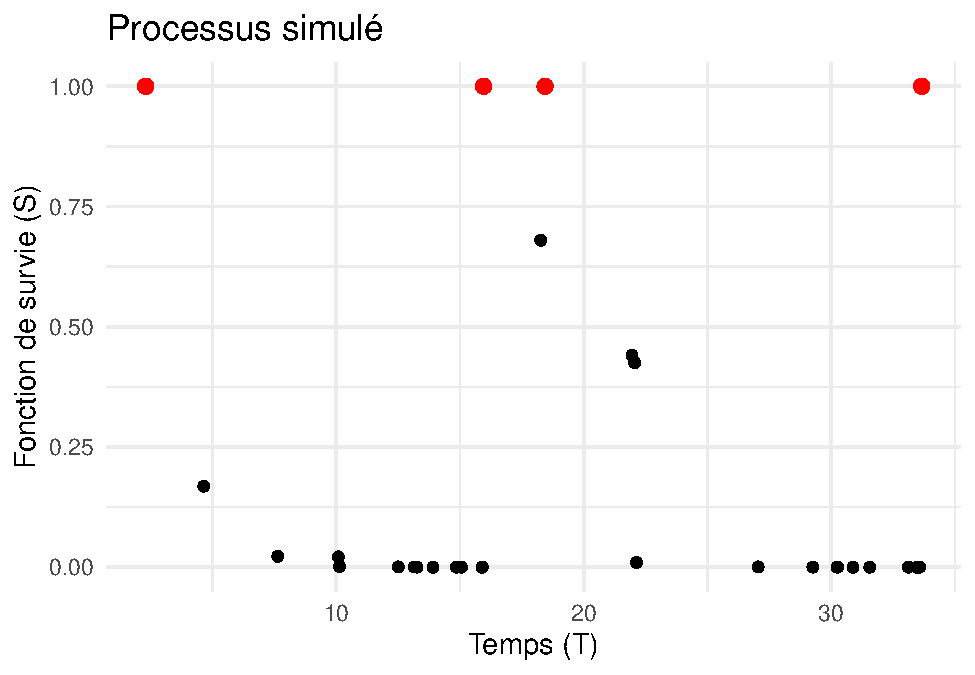
\includegraphics{Projet-Poisson_files/figure-latex/plot-1.pdf} On voit
donc que graphe est cohérent d'après les résulats des différents
vecteurs. En effet, lorsqu'il n'y a pas de réparations parfaites, l'âge
du système ne cesse d'augmenter et la valeur de la fonction de survie
tend vers 0 et à l'inverse, lorsqu'une réparation est parfaite, son âge
retombe à zéro et la fonction de survie vaut à nouveau 1.

\subsection{\texorpdfstring{Estimation du paramètre \(p\) par maximum de
vraisemblance}{Estimation du paramètre p par maximum de vraisemblance}}\label{estimation-du-paramuxe8tre-p-par-maximum-de-vraisemblance}

On implémente le calcul du MLE trouvé précedemment :\(\hat p=m/n\).

\begin{Shaded}
\begin{Highlighting}[]
\NormalTok{MLE\_P }\OtherTok{\textless{}{-}} \ControlFlowTok{function}\NormalTok{(m,n)}
\NormalTok{\{}
  \FunctionTok{return}\NormalTok{(m}\SpecialCharTok{/}\NormalTok{n)}
\NormalTok{\}}
\end{Highlighting}
\end{Shaded}

Pour observer le bon comportement de notre estimateur, on va simuler des
processus pour des valeurs de \(m\) croissantes et calculer à chaque
fois notre \(\hat p\).

\begin{Shaded}
\begin{Highlighting}[]
\NormalTok{p\_hat }\OtherTok{\textless{}{-}} \FunctionTok{c}\NormalTok{()}
\ControlFlowTok{for}\NormalTok{ (m }\ControlFlowTok{in} \DecValTok{1}\SpecialCharTok{:}\DecValTok{1000}\NormalTok{) \{}
\NormalTok{  process }\OtherTok{\textless{}{-}} \FunctionTok{simulPPIWeibull}\NormalTok{(m, }\DecValTok{1}\NormalTok{, }\DecValTok{2}\NormalTok{, }\FloatTok{0.2}\NormalTok{)}
\NormalTok{  p\_hat }\OtherTok{\textless{}{-}} \FunctionTok{c}\NormalTok{(p\_hat, m }\SpecialCharTok{/} \FunctionTok{length}\NormalTok{(process}\SpecialCharTok{$}\NormalTok{T))}
\NormalTok{\}}

\NormalTok{df }\OtherTok{\textless{}{-}} \FunctionTok{data.frame}\NormalTok{(}\AttributeTok{m =} \DecValTok{1}\SpecialCharTok{:}\DecValTok{1000}\NormalTok{, }\AttributeTok{p\_hat =}\NormalTok{ p\_hat)}

  \FunctionTok{ggplot}\NormalTok{(df, }\FunctionTok{aes}\NormalTok{(}\AttributeTok{x =}\NormalTok{ m, }\AttributeTok{y =}\NormalTok{ p\_hat)) }\SpecialCharTok{+}
    \FunctionTok{geom\_point}\NormalTok{(}\AttributeTok{color =} \StringTok{"blue"}\NormalTok{, }\AttributeTok{size =} \DecValTok{1}\NormalTok{) }\SpecialCharTok{+}       
    \FunctionTok{geom\_hline}\NormalTok{(}\AttributeTok{yintercept =} \FloatTok{0.2}\NormalTok{, }\AttributeTok{color =} \StringTok{"red"}\NormalTok{, }\AttributeTok{linetype =} \StringTok{"dashed"}\NormalTok{, }\AttributeTok{size =} \DecValTok{1}\NormalTok{) }\SpecialCharTok{+}  
    \FunctionTok{labs}\NormalTok{(}\AttributeTok{title =} \StringTok{"Estimation de p\_hat en fonction de m"}\NormalTok{,}
         \AttributeTok{x =} \StringTok{"m"}\NormalTok{,}
         \AttributeTok{y =} \StringTok{"p\_hat"}\NormalTok{) }\SpecialCharTok{+}
    \FunctionTok{theme\_minimal}\NormalTok{(}\AttributeTok{base\_size =} \DecValTok{14}\NormalTok{)}
\end{Highlighting}
\end{Shaded}

\begin{verbatim}
## Warning: Using `size` aesthetic for lines was deprecated in ggplot2 3.4.0.
## i Please use `linewidth` instead.
## This warning is displayed once every 8 hours.
## Call `lifecycle::last_lifecycle_warnings()` to see where this warning was
## generated.
\end{verbatim}

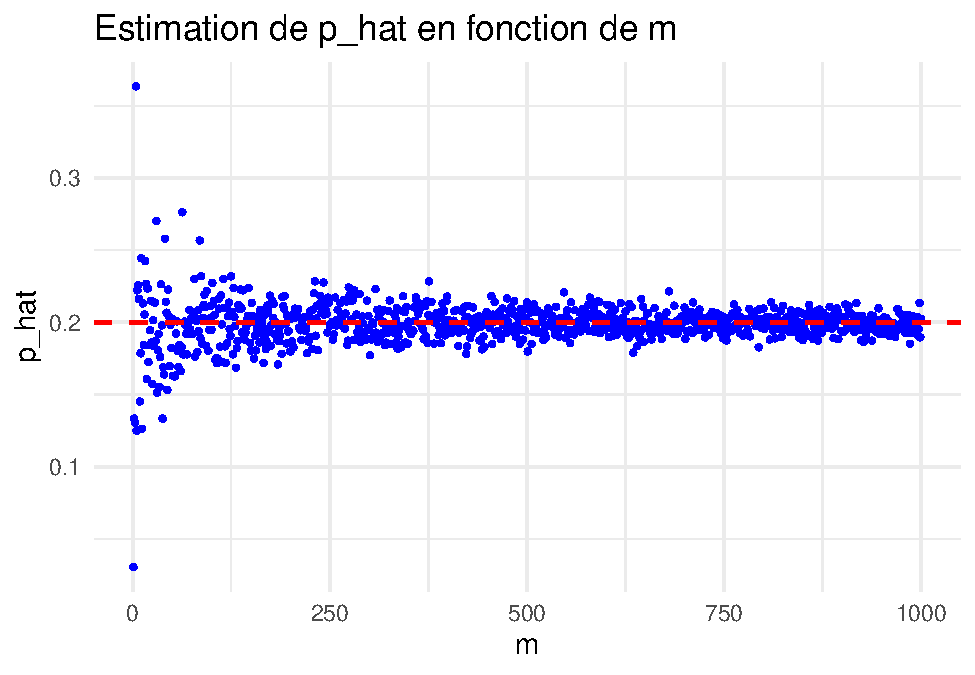
\includegraphics{Projet-Poisson_files/figure-latex/unnamed-chunk-1-1.pdf}
On observe que plus \(m\) augmente, plus notre estimation poctuelle se
rapproche de la vraie valeur de \(p\). On observe également que la
variance diminue.

\subsection{Estimation de l'intensité du processus par plusieurs
méthodes}\label{estimation-de-lintensituxe9-du-processus-par-plusieurs-muxe9thodes}

\subsubsection{Estimation par maximum de vraisemblance ou neighbourhood
MLE}\label{estimation-par-maximum-de-vraisemblance-ou-neighbourhood-mle}

On rappelle la formule du MLE qui est bien défini uniquement si
\(z_{(n-1)}=1\) (voir première partie du document): \[
\hat{S}(t) =
\left\{
\begin{array}{ll}
  1, & t < x_{(1)} \\
  \prod\limits_{j=1}^{i} \hat{\phi}_j, & x_{(i)} < t < x_{(i+1)}, \quad i=1,\dots,n-1 \\
  0, & t \geq x_{(n)}
\end{array}
\right.
\] On rappelle également que cet estimateur peut être utilisé pour
\(z_{(n-1)}=0\) mais devient un neighbourhood MLE et est nul pour
\(t\geq x_{(J+1)}\) où \(J\) est le dernier indice pour lequel
\(z_{(J)}=1\) (en dehors de \(z_{(n)}\)). On définit une nouvelle
fonction \(simulPPIWeibull2\), qui s'inspire fortement de la première
simulation mais qui ne renvoie pas les mêmes choses. Ici on retourne les
instants de pannes, la type de réparation associé à chaque panne
(\(=Z\)) ainsi que les instants de réparations parfaites (sous ensemble
de \(T\)).

\begin{Shaded}
\begin{Highlighting}[]
\NormalTok{simulPPIWeibull2 }\OtherTok{\textless{}{-}} \ControlFlowTok{function}\NormalTok{(m, alpha, beta, p)}
\NormalTok{\{}
\NormalTok{  k }\OtherTok{\textless{}{-}} \FunctionTok{rgeom}\NormalTok{(}\DecValTok{1}\NormalTok{, p)}\SpecialCharTok{+}\DecValTok{1}
\NormalTok{  A\_k }\OtherTok{=} \FunctionTok{simulPPh1}\NormalTok{(k)}
\NormalTok{  T\_k }\OtherTok{=} \FunctionTok{c}\NormalTok{(}\FunctionTok{invWeibull}\NormalTok{(A\_k, alpha, beta))}
\NormalTok{  Z\_k }\OtherTok{=} \FunctionTok{c}\NormalTok{(}\FunctionTok{rep}\NormalTok{(}\DecValTok{0}\NormalTok{,k}\DecValTok{{-}1}\NormalTok{),}\DecValTok{1}\NormalTok{)}
\NormalTok{  T\_succes }\OtherTok{=} \FunctionTok{tail}\NormalTok{(T\_k,}\DecValTok{1}\NormalTok{)}
  \ControlFlowTok{for}\NormalTok{(i }\ControlFlowTok{in} \DecValTok{1}\SpecialCharTok{:}\NormalTok{m}\DecValTok{{-}1}\NormalTok{)}
\NormalTok{  \{}
\NormalTok{   k }\OtherTok{\textless{}{-}} \FunctionTok{rgeom}\NormalTok{(}\DecValTok{1}\NormalTok{, p)}\SpecialCharTok{+}\DecValTok{1}
\NormalTok{   A\_k }\OtherTok{=} \FunctionTok{simulPPh1}\NormalTok{(k)}
\NormalTok{   T\_k\_temp }\OtherTok{=} \FunctionTok{c}\NormalTok{(}\FunctionTok{invWeibull}\NormalTok{(A\_k, alpha, beta))}
\NormalTok{   T\_k }\OtherTok{=} \FunctionTok{c}\NormalTok{(T\_k, }\FunctionTok{tail}\NormalTok{(T\_k,}\DecValTok{1}\NormalTok{) }\SpecialCharTok{+}\NormalTok{ T\_k\_temp)}
\NormalTok{   Z\_k }\OtherTok{=} \FunctionTok{c}\NormalTok{(Z\_k,}\FunctionTok{rep}\NormalTok{(}\DecValTok{0}\NormalTok{,k}\DecValTok{{-}1}\NormalTok{),}\DecValTok{1}\NormalTok{)}
\NormalTok{   T\_succes }\OtherTok{=} \FunctionTok{c}\NormalTok{(T\_succes, }\FunctionTok{tail}\NormalTok{(T\_k,}\DecValTok{1}\NormalTok{))}
\NormalTok{  \}}
  \FunctionTok{return}\NormalTok{(}\FunctionTok{list}\NormalTok{(}\AttributeTok{T =}\NormalTok{ T\_k,}\AttributeTok{Z=}\NormalTok{Z\_k, }\AttributeTok{T\_succes =}\NormalTok{ T\_succes))}
\NormalTok{\}}
\end{Highlighting}
\end{Shaded}

\begin{Shaded}
\begin{Highlighting}[]
\NormalTok{res}\OtherTok{\textless{}{-}}\FunctionTok{simulPPIWeibull2}\NormalTok{(}\DecValTok{50}\NormalTok{,}\DecValTok{4}\NormalTok{,}\DecValTok{2}\NormalTok{,}\FloatTok{0.2}\NormalTok{)}
\NormalTok{Z}\OtherTok{\textless{}{-}}\NormalTok{res}\SpecialCharTok{$}\NormalTok{Z}
\NormalTok{T}\OtherTok{\textless{}{-}}\NormalTok{res}\SpecialCharTok{$}\NormalTok{T }
\end{Highlighting}
\end{Shaded}

On implémente maintenant le calcul du MLE (ou neighbourhood MLE en
fonction des cas) trouvé précedemment. La fonction \(MLE_S\) renvoie les
vecteurs \(x_{()}\) et \(\hat \phi\) permettant de construire le MLE. On
a ensuite une deuxième fonction \(plot\_MLE\_S\) qui permet de
construire graphiquement le MLE en retournant ses valeurs pour une
séquence de temps \(t\).

\begin{Shaded}
\begin{Highlighting}[]
\NormalTok{MLE\_S }\OtherTok{\textless{}{-}} \ControlFlowTok{function}\NormalTok{(T,Z)}
\NormalTok{\{}
\NormalTok{  n}\OtherTok{\textless{}{-}}\FunctionTok{length}\NormalTok{(Z)}
\NormalTok{  x }\OtherTok{\textless{}{-}} \FunctionTok{c}\NormalTok{()}
\NormalTok{  last\_perfect }\OtherTok{\textless{}{-}} \DecValTok{0}
  \ControlFlowTok{for}\NormalTok{ (i }\ControlFlowTok{in} \DecValTok{1}\SpecialCharTok{:}\NormalTok{n)\{}
\NormalTok{    x }\OtherTok{\textless{}{-}} \FunctionTok{c}\NormalTok{(x,T[i]}\SpecialCharTok{{-}}\NormalTok{last\_perfect)}
  \ControlFlowTok{if}\NormalTok{ (Z[i]}\SpecialCharTok{==}\DecValTok{1}\NormalTok{)\{}
\NormalTok{    last\_perfect}\OtherTok{\textless{}{-}}\NormalTok{T[i]}
\NormalTok{  \}}
\NormalTok{  \}}
\NormalTok{  idx}\OtherTok{\textless{}{-}}\FunctionTok{order}\NormalTok{(x)}
\NormalTok{  x\_order}\OtherTok{\textless{}{-}}\NormalTok{x[idx]}
\NormalTok{  z\_order}\OtherTok{\textless{}{-}}\NormalTok{Z[idx]}
\NormalTok{  phi\_hat}\OtherTok{\textless{}{-}}\FunctionTok{c}\NormalTok{()}
  \ControlFlowTok{for}\NormalTok{ (i }\ControlFlowTok{in} \DecValTok{1}\SpecialCharTok{:}\NormalTok{(n}\DecValTok{{-}1}\NormalTok{))\{}
\NormalTok{    k}\OtherTok{\textless{}{-}}\FunctionTok{sum}\NormalTok{(z\_order[i}\SpecialCharTok{:}\NormalTok{(n}\DecValTok{{-}1}\NormalTok{)])}
\NormalTok{    phi\_hat}\OtherTok{\textless{}{-}}\FunctionTok{c}\NormalTok{(phi\_hat,k}\SpecialCharTok{/}\NormalTok{(k}\SpecialCharTok{+}\DecValTok{1}\NormalTok{))}
\NormalTok{  \}}
\NormalTok{  phi\_hat}\OtherTok{\textless{}{-}}\FunctionTok{c}\NormalTok{(phi\_hat,}\DecValTok{0}\NormalTok{)}
  \FunctionTok{return}\NormalTok{(}\FunctionTok{list}\NormalTok{(}\AttributeTok{x\_order =}\NormalTok{ x\_order,}\AttributeTok{phi\_hat=}\NormalTok{phi\_hat))}
\NormalTok{\}}
\NormalTok{plot\_MLE\_S }\OtherTok{\textless{}{-}}\ControlFlowTok{function}\NormalTok{(t,x\_order,phi\_hat) \{}
\NormalTok{  x\_order}\OtherTok{\textless{}{-}}\FunctionTok{c}\NormalTok{(x\_order,}\ConstantTok{Inf}\NormalTok{)}
\NormalTok{  S\_hat}\OtherTok{\textless{}{-}}\FunctionTok{rep}\NormalTok{(}\DecValTok{1}\NormalTok{,}\FunctionTok{length}\NormalTok{(t))}
  \CommentTok{\# Inférieur au premier temps de panne}
\NormalTok{  count}\OtherTok{\textless{}{-}}\DecValTok{1}
  \ControlFlowTok{while}\NormalTok{ (t[count]}\SpecialCharTok{\textless{}}\NormalTok{x\_order[}\DecValTok{1}\NormalTok{])\{}
\NormalTok{    count}\OtherTok{\textless{}{-}}\NormalTok{count}\SpecialCharTok{+}\DecValTok{1}
\NormalTok{  \}}
\NormalTok{  i}\OtherTok{\textless{}{-}}\DecValTok{1}
\NormalTok{  phi}\OtherTok{\textless{}{-}}\NormalTok{phi\_hat[}\DecValTok{1}\NormalTok{]}
  \CommentTok{\#Entre deux temps de pannes ou supérieur au dernier}
  \ControlFlowTok{for}\NormalTok{ (j }\ControlFlowTok{in}\NormalTok{ count}\SpecialCharTok{:}\FunctionTok{length}\NormalTok{(t))\{}
    \ControlFlowTok{if}\NormalTok{ (t[j]}\SpecialCharTok{\textgreater{}}\NormalTok{x\_order[i}\SpecialCharTok{+}\DecValTok{1}\NormalTok{])\{}
\NormalTok{      phi}\OtherTok{\textless{}{-}}\NormalTok{phi}\SpecialCharTok{*}\NormalTok{phi\_hat[i]}
\NormalTok{      i}\OtherTok{\textless{}{-}}\NormalTok{i}\SpecialCharTok{+}\DecValTok{1}
\NormalTok{    \}}
\NormalTok{    S\_hat[j]}\OtherTok{=}\NormalTok{phi}
\NormalTok{  \}}
  \FunctionTok{return}\NormalTok{(S\_hat)}
\NormalTok{\}}
\end{Highlighting}
\end{Shaded}

On teste le calcul et l'affichage de notre estimateur sur une simulation
simple.

\begin{Shaded}
\begin{Highlighting}[]
\NormalTok{r}\OtherTok{\textless{}{-}}\FunctionTok{MLE\_S}\NormalTok{(T,Z)}
\NormalTok{t}\OtherTok{\textless{}{-}}\FunctionTok{seq}\NormalTok{(}\DecValTok{0}\NormalTok{,}\DecValTok{10}\NormalTok{,}\FloatTok{0.01}\NormalTok{)}
\NormalTok{S\_hatBP }\OtherTok{\textless{}{-}} \FunctionTok{plot\_MLE\_S}\NormalTok{(t,r}\SpecialCharTok{$}\NormalTok{x\_order,r}\SpecialCharTok{$}\NormalTok{phi\_hat)}
\NormalTok{df }\OtherTok{\textless{}{-}} \FunctionTok{data.frame}\NormalTok{(}\AttributeTok{t =}\NormalTok{ t, }\AttributeTok{S\_hat =}\NormalTok{ S\_hatBP)}
\FunctionTok{ggplot}\NormalTok{(df, }\FunctionTok{aes}\NormalTok{(}\AttributeTok{x =}\NormalTok{ t, }\AttributeTok{y =}\NormalTok{ S\_hatBP)) }\SpecialCharTok{+}
  \FunctionTok{geom\_point}\NormalTok{(}\AttributeTok{color =} \StringTok{"black"}\NormalTok{, }\AttributeTok{size =} \DecValTok{1}\NormalTok{) }\SpecialCharTok{+}       
  \FunctionTok{geom\_line}\NormalTok{()}\SpecialCharTok{+}
  \FunctionTok{labs}\NormalTok{(}\AttributeTok{title =} \StringTok{"Estimation de S en fonction du temps"}\NormalTok{,}
       \AttributeTok{x =} \StringTok{"t"}\NormalTok{,}
       \AttributeTok{y =} \StringTok{"S"}\NormalTok{) }\SpecialCharTok{+}
  \FunctionTok{theme\_minimal}\NormalTok{(}\AttributeTok{base\_size =} \DecValTok{14}\NormalTok{)}
\end{Highlighting}
\end{Shaded}

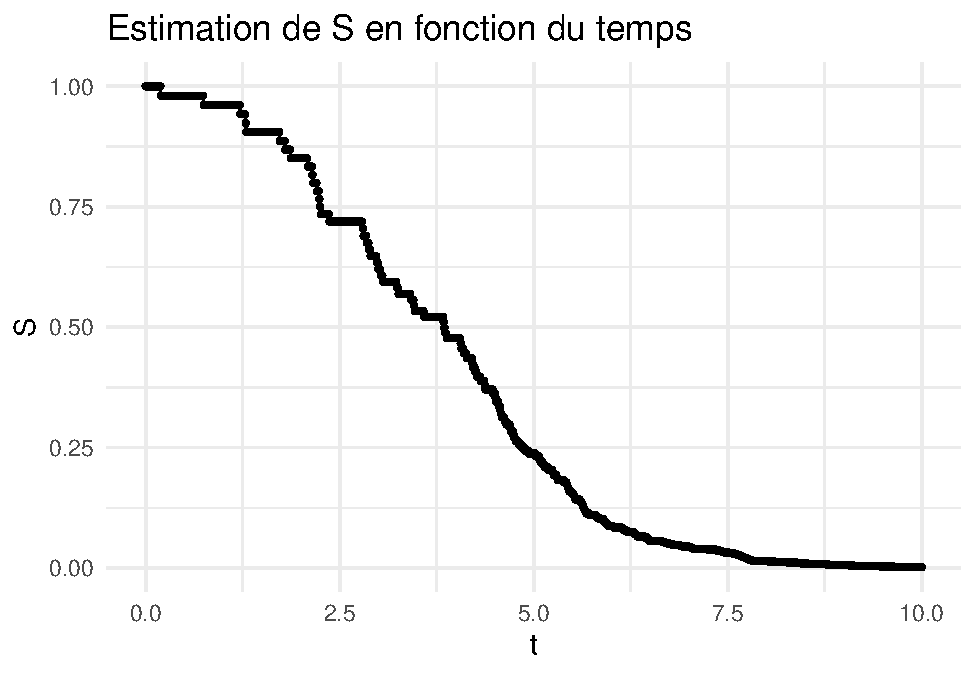
\includegraphics{Projet-Poisson_files/figure-latex/unnamed-chunk-5-1.pdf}

\subsubsection{Estimation de l'intensité du processus en utilisant les
temps de pannes à la suite d'une réparation
parfaite}\label{estimation-de-lintensituxe9-du-processus-en-utilisant-les-temps-de-pannes-uxe0-la-suite-dune-ruxe9paration-parfaite}

On va maintenant utiliser la distribution empirique des
\(T_i | Z_{i-1} = 1\), c'est-à-dire des durées entre chaque réparation
parfaite et la réparation suivante pour obtenir une approximation de la
densité. En la cumulant, on obtient une estimation de la fonction de
répartition. On définit comme avant 2 fonctions, une nous retournant
tout le nécessaire pour construire l'estimateur et une seconde pour
construire l'estimateur et retourner les valeurs en une séquence de
temps \(t\) donnée.

\begin{Shaded}
\begin{Highlighting}[]
\NormalTok{MLE\_emp\_1 }\OtherTok{\textless{}{-}} \ControlFlowTok{function}\NormalTok{(T,Z)}
\NormalTok{\{}
\NormalTok{  n}\OtherTok{\textless{}{-}}\FunctionTok{length}\NormalTok{(Z)}
\NormalTok{  delta\_t }\OtherTok{\textless{}{-}} \FunctionTok{c}\NormalTok{()}
\NormalTok{  last\_perfect }\OtherTok{\textless{}{-}} \DecValTok{0}
  \ControlFlowTok{for}\NormalTok{ (i }\ControlFlowTok{in} \DecValTok{1}\SpecialCharTok{:}\NormalTok{(n}\DecValTok{{-}1}\NormalTok{))\{}
    \ControlFlowTok{if}\NormalTok{(Z[i]}\SpecialCharTok{==}\DecValTok{1}\NormalTok{)\{}
\NormalTok{      delta\_t }\OtherTok{\textless{}{-}} \FunctionTok{c}\NormalTok{(delta\_t,T[i}\SpecialCharTok{+}\DecValTok{1}\NormalTok{]}\SpecialCharTok{{-}}\NormalTok{T[i])}
\NormalTok{    \}}
\NormalTok{  \}}
\NormalTok{  idd}\OtherTok{\textless{}{-}}\FunctionTok{order}\NormalTok{(delta\_t)}
\NormalTok{  delta\_t\_ordered }\OtherTok{\textless{}{-}}\NormalTok{ delta\_t[idd]}
  \FunctionTok{return}\NormalTok{(delta\_t\_ordered)}
\NormalTok{\}}

\NormalTok{plot\_MLE\_emp\_1 }\OtherTok{\textless{}{-}} \ControlFlowTok{function}\NormalTok{(t, x)}
\NormalTok{\{}
\NormalTok{  num\_perfect }\OtherTok{\textless{}{-}} \FunctionTok{length}\NormalTok{(x)}
\NormalTok{  x}\OtherTok{\textless{}{-}}\FunctionTok{c}\NormalTok{(x,}\ConstantTok{Inf}\NormalTok{)}
\NormalTok{  S\_hat}\OtherTok{\textless{}{-}}\FunctionTok{rep}\NormalTok{(}\DecValTok{1}\NormalTok{,}\FunctionTok{length}\NormalTok{(t))}
  \CommentTok{\# Inférieur au premier temps de panne}
\NormalTok{  count}\OtherTok{\textless{}{-}}\DecValTok{1}
  \ControlFlowTok{while}\NormalTok{ (t[count]}\SpecialCharTok{\textless{}}\NormalTok{x[}\DecValTok{1}\NormalTok{])\{}
\NormalTok{    S\_hat[count] }\OtherTok{\textless{}{-}} \DecValTok{1}
\NormalTok{    count}\OtherTok{\textless{}{-}}\NormalTok{count}\SpecialCharTok{+}\DecValTok{1}
\NormalTok{  \}}
\NormalTok{  i}\OtherTok{\textless{}{-}}\DecValTok{1}
\NormalTok{  S\_hat[count]}\OtherTok{\textless{}{-}}\NormalTok{(num\_perfect }\SpecialCharTok{{-}} \DecValTok{1}\NormalTok{)}\SpecialCharTok{/}\NormalTok{num\_perfect}
  \CommentTok{\#Entre deux temps de pannes ou supérieur au dernier}
  \ControlFlowTok{for}\NormalTok{ (j }\ControlFlowTok{in}\NormalTok{ count}\SpecialCharTok{:}\FunctionTok{length}\NormalTok{(t))\{}
    \ControlFlowTok{if}\NormalTok{ (t[j]}\SpecialCharTok{\textgreater{}}\NormalTok{x[i}\SpecialCharTok{+}\DecValTok{1}\NormalTok{])\{}
\NormalTok{      i}\OtherTok{\textless{}{-}}\NormalTok{i}\SpecialCharTok{+}\DecValTok{1}
\NormalTok{    \}}
\NormalTok{    S\_hat[j]}\OtherTok{=}\NormalTok{(num\_perfect }\SpecialCharTok{{-}}\NormalTok{ i)}\SpecialCharTok{/}\NormalTok{num\_perfect}
\NormalTok{  \}}
  \FunctionTok{return}\NormalTok{(S\_hat)}
\NormalTok{\}}
\end{Highlighting}
\end{Shaded}

On teste l'affichage de l'estimateur sur la même simulation que
l'estimateur précédent.

\begin{Shaded}
\begin{Highlighting}[]
\NormalTok{idd}\OtherTok{\textless{}{-}}\FunctionTok{MLE\_emp\_1}\NormalTok{(T,Z)}
\NormalTok{idd}
\end{Highlighting}
\end{Shaded}

\begin{verbatim}
##  [1] 0.9917336 1.0615283 1.1219341 1.1768976 1.2064476 1.3063846 1.7748335
##  [8] 2.1302691 2.5851749 2.5961483 2.7565007 2.9438525 3.0588314 3.2283112
## [15] 3.2305251 3.2484997 3.2779147 3.3019153 3.3172099 3.4620854 3.4801944
## [22] 3.5660021 3.6419064 3.7808839 3.8089303 3.8377450 3.9123744 3.9866404
## [29] 4.1788458 4.2615219 4.5451060 4.5926212 4.6211045 4.8601034 4.8679230
## [36] 5.0224089 5.1365522 5.2477365 5.4643229 5.8739386 5.8923122 5.9748825
## [43] 6.1728359 6.1956036 6.3752632 6.8046722 7.2519776 7.3718260 7.5565930
## [50] 8.8812373
\end{verbatim}

\begin{Shaded}
\begin{Highlighting}[]
\NormalTok{S\_hat\_e1 }\OtherTok{\textless{}{-}} \FunctionTok{plot\_MLE\_emp\_1}\NormalTok{(t,idd)}
\NormalTok{df }\OtherTok{\textless{}{-}} \FunctionTok{data.frame}\NormalTok{(}\AttributeTok{t =}\NormalTok{ t, }\AttributeTok{S\_hat\_e1 =}\NormalTok{S\_hat\_e1)}
\FunctionTok{ggplot}\NormalTok{(df, }\FunctionTok{aes}\NormalTok{(}\AttributeTok{x =}\NormalTok{ t, }\AttributeTok{y =}\NormalTok{S\_hat\_e1)) }\SpecialCharTok{+}
  \FunctionTok{geom\_point}\NormalTok{(}\AttributeTok{color =} \StringTok{"black"}\NormalTok{, }\AttributeTok{size =} \DecValTok{1}\NormalTok{) }\SpecialCharTok{+}       
  \FunctionTok{geom\_line}\NormalTok{()}\SpecialCharTok{+}
  \FunctionTok{labs}\NormalTok{(}\AttributeTok{title =} \StringTok{"Estimation de S en fonction du temps (estimateur empirique 1)"}\NormalTok{,}
       \AttributeTok{x =} \StringTok{"t"}\NormalTok{,}
       \AttributeTok{y =} \StringTok{"S"}\NormalTok{) }\SpecialCharTok{+}
  \FunctionTok{theme\_minimal}\NormalTok{(}\AttributeTok{base\_size =} \DecValTok{14}\NormalTok{)}
\end{Highlighting}
\end{Shaded}

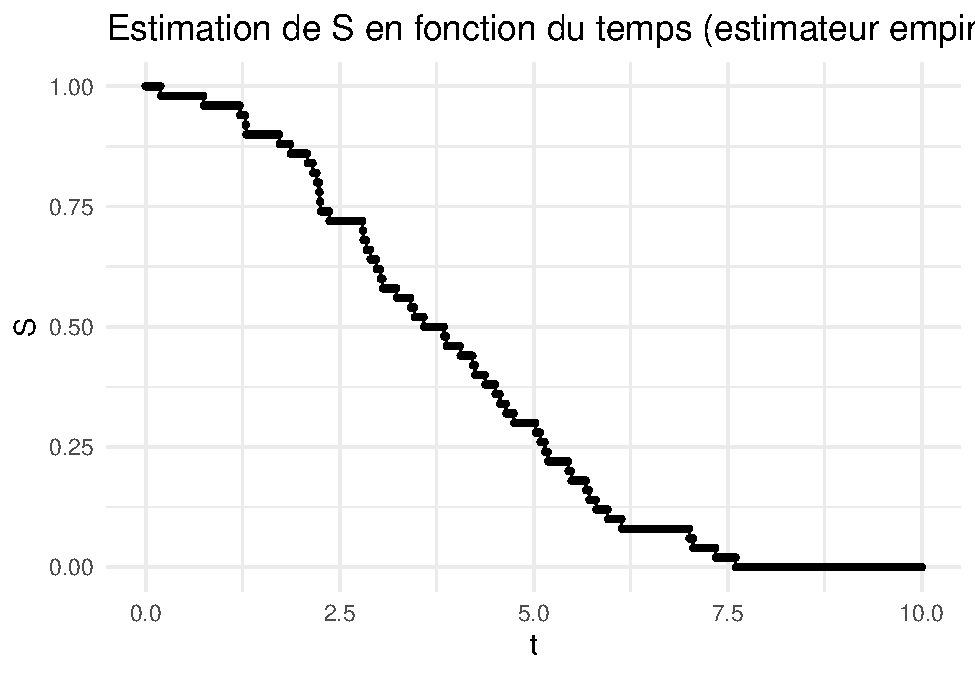
\includegraphics{Projet-Poisson_files/figure-latex/unnamed-chunk-7-1.pdf}

\subsubsection{Estimation de l'intensité du processus avec uniquement
les temps de réparations
parfaites}\label{estimation-de-lintensituxe9-du-processus-avec-uniquement-les-temps-de-ruxe9parations-parfaites}

On va maintenant utiliser la distribution empirique du processus de
Poisson inhomogène obtenu en ne considérant que les durées entre deux
réparations parfaites \(Y_1\), \ldots{} , \(Y_m\). On obtient ainsi une
approximation de \(S_y\), que l'on note \(\hat S_y\). Or
\(S_y(t)=(S(t))^p\), donc on obtient via \(1 - \hat S_y ^{n/m}\) notre
estimateur de la fonction de répartition. On reprend les mêmes
conventions de codes que pour les deux estimateurs précédent.

\begin{Shaded}
\begin{Highlighting}[]
\NormalTok{MLE\_emp\_2\_c }\OtherTok{\textless{}{-}} \ControlFlowTok{function}\NormalTok{(T,Z)}
\NormalTok{\{}
\NormalTok{  n}\OtherTok{\textless{}{-}}\FunctionTok{length}\NormalTok{(Z)}
\NormalTok{  perfects }\OtherTok{\textless{}{-}} \FunctionTok{c}\NormalTok{()}
\NormalTok{  last\_perfect }\OtherTok{\textless{}{-}} \DecValTok{0}
  \ControlFlowTok{for}\NormalTok{ (i }\ControlFlowTok{in} \DecValTok{1}\SpecialCharTok{:}\NormalTok{n)\{}
    \ControlFlowTok{if}\NormalTok{(Z[i]}\SpecialCharTok{==}\DecValTok{1}\NormalTok{)\{}
\NormalTok{      perfects }\OtherTok{\textless{}{-}} \FunctionTok{c}\NormalTok{(perfects,T[i])}
\NormalTok{    \}}
\NormalTok{  \}}
\NormalTok{  inter\_perfects }\OtherTok{\textless{}{-}} \FunctionTok{c}\NormalTok{()}
\NormalTok{  inter\_perfects }\OtherTok{\textless{}{-}} \FunctionTok{c}\NormalTok{(perfects[}\DecValTok{1}\NormalTok{])}
  \ControlFlowTok{for}\NormalTok{ (i }\ControlFlowTok{in} \DecValTok{1}\SpecialCharTok{:}\FunctionTok{length}\NormalTok{(perfects)}\SpecialCharTok{{-}}\DecValTok{1}\NormalTok{)\{}
\NormalTok{    inter\_perfects }\OtherTok{\textless{}{-}} \FunctionTok{c}\NormalTok{(inter\_perfects, perfects[i}\SpecialCharTok{+}\DecValTok{1}\NormalTok{] }\SpecialCharTok{{-}}\NormalTok{ perfects[i])}
\NormalTok{  \}}
\NormalTok{  idd}\OtherTok{\textless{}{-}}\FunctionTok{order}\NormalTok{(inter\_perfects)}
\NormalTok{  inter\_perfects\_ordered }\OtherTok{\textless{}{-}}\NormalTok{ inter\_perfects[idd]}
  \FunctionTok{return}\NormalTok{(inter\_perfects\_ordered)}
\NormalTok{\}}

\NormalTok{plot\_MLE\_emp\_2 }\OtherTok{\textless{}{-}} \ControlFlowTok{function}\NormalTok{(t, ipo, Z)}
\NormalTok{\{}
\NormalTok{  num\_repairs }\OtherTok{\textless{}{-}} \FunctionTok{length}\NormalTok{(Z)}
\NormalTok{  num\_perfect }\OtherTok{\textless{}{-}} \FunctionTok{length}\NormalTok{(ipo)}
\NormalTok{  ipo}\OtherTok{\textless{}{-}}\FunctionTok{c}\NormalTok{(ipo,}\ConstantTok{Inf}\NormalTok{)}
\NormalTok{  S\_hat\_y}\OtherTok{\textless{}{-}}\FunctionTok{rep}\NormalTok{(}\DecValTok{1}\NormalTok{,}\FunctionTok{length}\NormalTok{(t))}
  \CommentTok{\# Inférieur au premier temps de panne}
\NormalTok{  count}\OtherTok{\textless{}{-}}\DecValTok{1}
  \ControlFlowTok{while}\NormalTok{ (t[count]}\SpecialCharTok{\textless{}}\NormalTok{ipo[}\DecValTok{1}\NormalTok{])\{}
\NormalTok{    S\_hat\_y[count] }\OtherTok{\textless{}{-}} \DecValTok{1}
\NormalTok{    count}\OtherTok{\textless{}{-}}\NormalTok{count}\SpecialCharTok{+}\DecValTok{1}
\NormalTok{  \}}
\NormalTok{  i}\OtherTok{\textless{}{-}}\DecValTok{1}
\NormalTok{  S\_hat\_y[count]}\OtherTok{\textless{}{-}}\NormalTok{(num\_perfect }\SpecialCharTok{{-}} \DecValTok{1}\NormalTok{)}\SpecialCharTok{/}\NormalTok{num\_perfect}
  \CommentTok{\#Entre deux temps de pannes ou supérieur au dernier}
  \ControlFlowTok{for}\NormalTok{ (j }\ControlFlowTok{in}\NormalTok{ (count}\SpecialCharTok{+}\DecValTok{1}\NormalTok{)}\SpecialCharTok{:}\FunctionTok{length}\NormalTok{(t))\{}
    \ControlFlowTok{if}\NormalTok{ (t[j]}\SpecialCharTok{\textgreater{}}\NormalTok{ipo[i}\SpecialCharTok{+}\DecValTok{1}\NormalTok{])\{}
\NormalTok{      i}\OtherTok{\textless{}{-}}\NormalTok{i}\SpecialCharTok{+}\DecValTok{1}
\NormalTok{    \}}
\NormalTok{    S\_hat\_y[j]}\OtherTok{=}\NormalTok{(num\_perfect }\SpecialCharTok{{-}}\NormalTok{ i)}\SpecialCharTok{/}\NormalTok{num\_perfect}
\NormalTok{  \}}
  
\NormalTok{  S\_hat }\OtherTok{\textless{}{-}}\NormalTok{ (S\_hat\_y)}\SpecialCharTok{**}\NormalTok{(num\_repairs }\SpecialCharTok{/}\NormalTok{ num\_perfect)}
  
  \FunctionTok{return}\NormalTok{(S\_hat)}
\NormalTok{\}}
\end{Highlighting}
\end{Shaded}

On teste l'affichage de l'estimateur sur la même simulation que pour les
estimateurs précédents.

\begin{Shaded}
\begin{Highlighting}[]
\NormalTok{ipo}\OtherTok{\textless{}{-}}\FunctionTok{MLE\_emp\_2\_c}\NormalTok{(T,Z)}
\NormalTok{ipo}
\end{Highlighting}
\end{Shaded}

\begin{verbatim}
##  [1]  1.910856  3.301915  3.641906  4.501862  4.631583  4.740300  5.005251
##  [8]  5.174509  5.247736  5.373704  5.711218  5.869472  6.015139  6.172836
## [15]  6.263241  6.281800  6.612213  6.667082  6.990219  7.035976  7.222092
## [22]  7.285791  7.371826  7.732284  7.754713  8.052654  8.141829  8.391337
## [29]  8.542591  8.571159  8.650720  8.671102  8.858611  9.109813  9.554122
## [36]  9.666943 10.663787 10.742672 10.883221 10.912433 10.919018 11.277142
## [43] 11.508491 11.860724 12.406735 13.029500 13.187027 13.444986 16.077566
## [50] 18.409980 18.527291
\end{verbatim}

\begin{Shaded}
\begin{Highlighting}[]
\NormalTok{S\_hat\_e2 }\OtherTok{\textless{}{-}} \FunctionTok{plot\_MLE\_emp\_2}\NormalTok{(t,ipo, Z)}
\NormalTok{df }\OtherTok{\textless{}{-}} \FunctionTok{data.frame}\NormalTok{(}\AttributeTok{t =}\NormalTok{ t, }\AttributeTok{S\_hat\_e2 =}\NormalTok{S\_hat\_e2)}
\FunctionTok{ggplot}\NormalTok{(df, }\FunctionTok{aes}\NormalTok{(}\AttributeTok{x =}\NormalTok{ t, }\AttributeTok{y =}\NormalTok{S\_hat\_e2)) }\SpecialCharTok{+}
  \FunctionTok{geom\_point}\NormalTok{(}\AttributeTok{color =} \StringTok{"black"}\NormalTok{, }\AttributeTok{size =} \DecValTok{1}\NormalTok{) }\SpecialCharTok{+}       
  \FunctionTok{geom\_line}\NormalTok{()}\SpecialCharTok{+}
  \FunctionTok{labs}\NormalTok{(}\AttributeTok{title =} \StringTok{"Estimation de S en fonction du temps (estimateur empirique 2)"}\NormalTok{,}
       \AttributeTok{x =} \StringTok{"t"}\NormalTok{,}
       \AttributeTok{y =} \StringTok{"S"}\NormalTok{) }\SpecialCharTok{+}
  \FunctionTok{theme\_minimal}\NormalTok{(}\AttributeTok{base\_size =} \DecValTok{14}\NormalTok{)}
\end{Highlighting}
\end{Shaded}

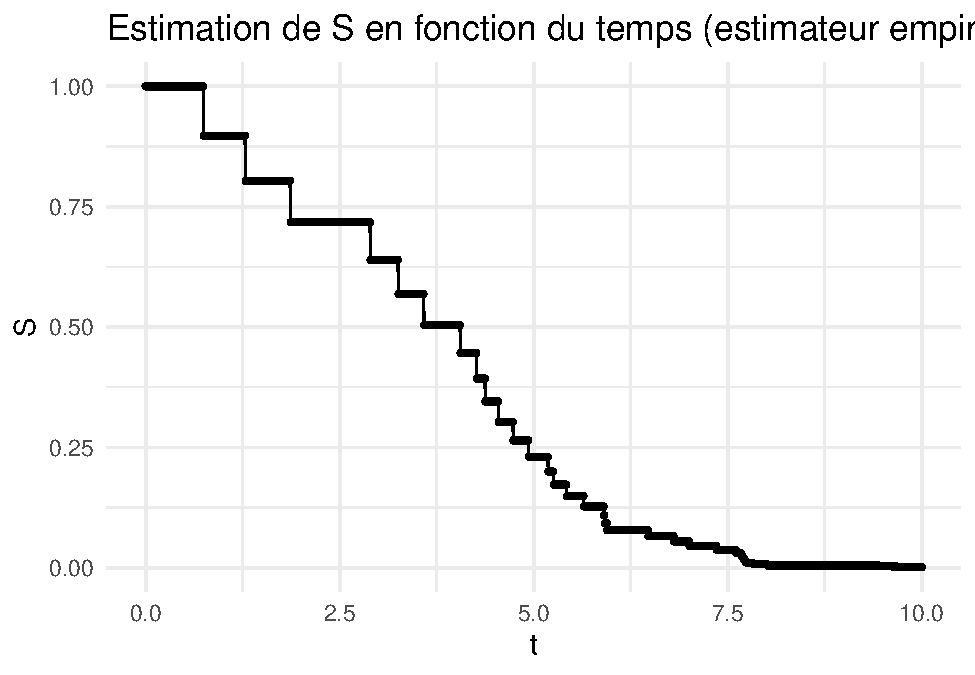
\includegraphics{Projet-Poisson_files/figure-latex/unnamed-chunk-9-1.pdf}

\subsubsection{Comparaison des
estimateurs}\label{comparaison-des-estimateurs}

Pour comparer nos estimateurs de la fonction de survie \(S\), on va
évaluer la fonction de survie théorique d'un processus de Weibull, que
l'on peut calculer, en une séquence de temps positifs. On va ensuite
afficher sur le même graphe cette courbe exacte et celles obtenues avec
chacun des estimateurs.

\begin{Shaded}
\begin{Highlighting}[]
\NormalTok{SWeibull }\OtherTok{\textless{}{-}} \ControlFlowTok{function}\NormalTok{(y, }\AttributeTok{alpha=}\DecValTok{1}\NormalTok{, }\AttributeTok{beta=}\DecValTok{2}\NormalTok{)}
\NormalTok{\{}
  \FunctionTok{return}\NormalTok{(}\FunctionTok{exp}\NormalTok{(}\SpecialCharTok{{-}}\NormalTok{(y}\SpecialCharTok{/}\NormalTok{alpha)}\SpecialCharTok{**}\NormalTok{beta))}
\NormalTok{\}}
\end{Highlighting}
\end{Shaded}

\begin{Shaded}
\begin{Highlighting}[]
\NormalTok{df }\OtherTok{\textless{}{-}} \FunctionTok{data.frame}\NormalTok{(}
  \AttributeTok{t =}\NormalTok{ t,}
  \AttributeTok{SWeibull =} \FunctionTok{SWeibull}\NormalTok{(t, }\DecValTok{4}\NormalTok{, }\DecValTok{2}\NormalTok{),}
  \AttributeTok{BP =}\NormalTok{ S\_hatBP,}
  \AttributeTok{e1 =}\NormalTok{ S\_hat\_e1,}
  \AttributeTok{e2 =}\NormalTok{ S\_hat\_e2}
\NormalTok{)}

\NormalTok{df\_long }\OtherTok{\textless{}{-}}\NormalTok{ df }\SpecialCharTok{\%\textgreater{}\%}
  \FunctionTok{pivot\_longer}\NormalTok{(}\AttributeTok{cols =} \SpecialCharTok{{-}}\NormalTok{t, }\AttributeTok{names\_to =} \StringTok{"Méthode"}\NormalTok{, }\AttributeTok{values\_to =} \StringTok{"Survie"}\NormalTok{)}

\CommentTok{\# Plot}
\FunctionTok{ggplot}\NormalTok{(df\_long, }\FunctionTok{aes}\NormalTok{(}\AttributeTok{x =}\NormalTok{ t, }\AttributeTok{y =}\NormalTok{ Survie, }\AttributeTok{color =}\NormalTok{ Méthode)) }\SpecialCharTok{+}
  \FunctionTok{geom\_line}\NormalTok{(}\AttributeTok{size =} \FloatTok{1.2}\NormalTok{,}\AttributeTok{alpha =} \FloatTok{0.6}\NormalTok{) }\SpecialCharTok{+}
  \FunctionTok{labs}\NormalTok{(}\AttributeTok{title =} \StringTok{"Comparaison des courbes de survie"}\NormalTok{,}
       \AttributeTok{x =} \StringTok{"Temps"}\NormalTok{,}
       \AttributeTok{y =} \StringTok{"Fonction de survie S(t)"}\NormalTok{,}
       \AttributeTok{color =} \StringTok{"Méthode"}\NormalTok{) }\SpecialCharTok{+}
  \FunctionTok{theme\_minimal}\NormalTok{(}\AttributeTok{base\_size =} \DecValTok{14}\NormalTok{)}
\end{Highlighting}
\end{Shaded}

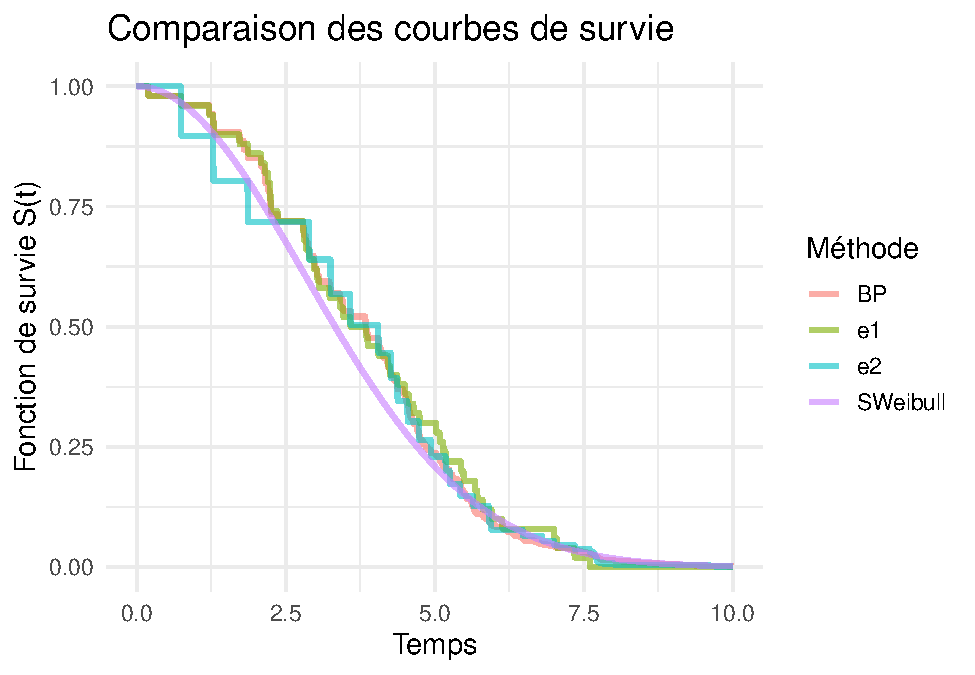
\includegraphics{Projet-Poisson_files/figure-latex/Comparaison_visuelle-1.pdf}
En plus de ce critère graphique qui permet une identification visuelle
de la performance, on va implémenter 2 critères numériques, la MSE et la
variance en fonction du nombre de réparations parfaites \(m\).

\begin{Shaded}
\begin{Highlighting}[]
\NormalTok{nrpm }\OtherTok{\textless{}{-}} \DecValTok{100} \CommentTok{\# Nombre de réparations parfaites max}
\NormalTok{mse\_BP }\OtherTok{\textless{}{-}} \FunctionTok{c}\NormalTok{()}
\NormalTok{mse\_e1 }\OtherTok{\textless{}{-}} \FunctionTok{c}\NormalTok{()}
\NormalTok{mse\_e2 }\OtherTok{\textless{}{-}} \FunctionTok{c}\NormalTok{()}
\ControlFlowTok{for}\NormalTok{ (m }\ControlFlowTok{in} \DecValTok{5}\SpecialCharTok{:}\NormalTok{nrpm)\{}
\NormalTok{  res}\OtherTok{\textless{}{-}}\FunctionTok{simulPPIWeibull2}\NormalTok{(m,}\DecValTok{4}\NormalTok{,}\DecValTok{2}\NormalTok{,}\FloatTok{0.1}\NormalTok{)}
\NormalTok{  Z}\OtherTok{\textless{}{-}}\NormalTok{res}\SpecialCharTok{$}\NormalTok{Z}
\NormalTok{  T}\OtherTok{\textless{}{-}}\NormalTok{res}\SpecialCharTok{$}\NormalTok{T}
\NormalTok{  t}\OtherTok{\textless{}{-}}\FunctionTok{seq}\NormalTok{(}\DecValTok{0}\NormalTok{,}\DecValTok{10}\NormalTok{,}\FloatTok{0.1}\SpecialCharTok{*}\DecValTok{1}\SpecialCharTok{/}\NormalTok{m)}
\NormalTok{  S\_t }\OtherTok{\textless{}{-}} \FunctionTok{SWeibull}\NormalTok{(t, }\DecValTok{4}\NormalTok{,}\DecValTok{2}\NormalTok{)}
\NormalTok{  r}\OtherTok{\textless{}{-}}\FunctionTok{MLE\_S}\NormalTok{(T,Z)}
\NormalTok{  S\_hatBP }\OtherTok{\textless{}{-}} \FunctionTok{plot\_MLE\_S}\NormalTok{(t,r}\SpecialCharTok{$}\NormalTok{x\_order,r}\SpecialCharTok{$}\NormalTok{phi\_hat)}
\NormalTok{  idd}\OtherTok{\textless{}{-}}\FunctionTok{MLE\_emp\_1}\NormalTok{(T,Z)}
\NormalTok{  S\_hat\_e1 }\OtherTok{\textless{}{-}} \FunctionTok{plot\_MLE\_emp\_1}\NormalTok{(t,idd)}
\NormalTok{  ipo}\OtherTok{\textless{}{-}}\FunctionTok{MLE\_emp\_2\_c}\NormalTok{(T,Z)}
\NormalTok{  S\_hat\_e2 }\OtherTok{\textless{}{-}} \FunctionTok{plot\_MLE\_emp\_2}\NormalTok{(t,ipo, Z)}
\NormalTok{  mse\_BP }\OtherTok{\textless{}{-}} \FunctionTok{c}\NormalTok{(mse\_BP, }\FunctionTok{sum}\NormalTok{((S\_t }\SpecialCharTok{{-}}\NormalTok{ S\_hatBP)}\SpecialCharTok{**}\DecValTok{2}\NormalTok{)}\SpecialCharTok{/}\FunctionTok{length}\NormalTok{(S\_t))}
\NormalTok{  mse\_e1 }\OtherTok{\textless{}{-}} \FunctionTok{c}\NormalTok{(mse\_e1, }\FunctionTok{sum}\NormalTok{((S\_t }\SpecialCharTok{{-}}\NormalTok{ S\_hat\_e1)}\SpecialCharTok{**}\DecValTok{2}\NormalTok{)}\SpecialCharTok{/}\FunctionTok{length}\NormalTok{(S\_t))}
\NormalTok{  mse\_e2 }\OtherTok{\textless{}{-}} \FunctionTok{c}\NormalTok{(mse\_e2, }\FunctionTok{sum}\NormalTok{((S\_t }\SpecialCharTok{{-}}\NormalTok{ S\_hat\_e2)}\SpecialCharTok{**}\DecValTok{2}\NormalTok{)}\SpecialCharTok{/}\FunctionTok{length}\NormalTok{(S\_t))}
\NormalTok{\}}
\end{Highlighting}
\end{Shaded}

\begin{Shaded}
\begin{Highlighting}[]
\NormalTok{df\_mse }\OtherTok{\textless{}{-}} \FunctionTok{data.frame}\NormalTok{(}
  \AttributeTok{m =} \FunctionTok{seq}\NormalTok{(}\DecValTok{5}\NormalTok{,nrpm),}
  \AttributeTok{BP =} \FunctionTok{log}\NormalTok{(mse\_BP),}
  \AttributeTok{e1 =} \FunctionTok{log}\NormalTok{(mse\_e1),}
  \AttributeTok{e2 =} \FunctionTok{log}\NormalTok{(mse\_e2)}
\NormalTok{)}

\NormalTok{df\_mse\_long }\OtherTok{\textless{}{-}}\NormalTok{ df\_mse }\SpecialCharTok{\%\textgreater{}\%}
  \FunctionTok{pivot\_longer}\NormalTok{(}\AttributeTok{cols =} \SpecialCharTok{{-}}\NormalTok{m, }\AttributeTok{names\_to =} \StringTok{"Méthode"}\NormalTok{, }\AttributeTok{values\_to =} \StringTok{"log\_MSE"}\NormalTok{)}

\FunctionTok{ggplot}\NormalTok{(df\_mse\_long, }\FunctionTok{aes}\NormalTok{(}\AttributeTok{x =}\NormalTok{ m, }\AttributeTok{y =}\NormalTok{ log\_MSE, }\AttributeTok{color =}\NormalTok{ Méthode)) }\SpecialCharTok{+}
  \FunctionTok{geom\_line}\NormalTok{(}\AttributeTok{size =} \FloatTok{1.2}\NormalTok{, }\AttributeTok{alpha =} \FloatTok{0.8}\NormalTok{) }\SpecialCharTok{+}
  \FunctionTok{labs}\NormalTok{(}\AttributeTok{title =} \StringTok{"Évolution du log(MSE) selon la méthode"}\NormalTok{,}
       \AttributeTok{x =} \StringTok{"Nombre de réparations parfaites"}\NormalTok{,}
       \AttributeTok{y =} \StringTok{"log(MSE)"}\NormalTok{,}
       \AttributeTok{color =} \StringTok{"Méthode"}\NormalTok{) }\SpecialCharTok{+}
  \FunctionTok{theme\_minimal}\NormalTok{(}\AttributeTok{base\_size =} \DecValTok{14}\NormalTok{)}
\end{Highlighting}
\end{Shaded}

\includegraphics{Projet-Poisson_files/figure-latex/Plot Comparaison_numérique-1.pdf}

On voit que l'estimateur du MLE non paramétrique, qui est celui qui
utilise le plus d'informations, mais qui ne possède pas de garanties
théoriques en l'absence de \(z_{n-1} = z_{n} = 1\), est celui qui
possède les meilleures performances pour la majorité des simulations.
C'est un résultat particulièrement visible lorsque les réparations
parfaites sont assez rares comparées aux réparations imparfaites. On
observe également que l'erreur des estimateurs à tendance à diminuer
lorsqu'on augmente le nombre de réparations (via l'augmentations du
nombre de réparations parfaites).

\begin{Shaded}
\begin{Highlighting}[]
\NormalTok{nrpm }\OtherTok{\textless{}{-}} \DecValTok{100} \CommentTok{\# Nombre de réparations parfaites max}
\NormalTok{niter }\OtherTok{\textless{}{-}} \DecValTok{10}
\NormalTok{var\_BP }\OtherTok{\textless{}{-}} \FunctionTok{rep}\NormalTok{(}\DecValTok{0}\NormalTok{,nrpm)}
\NormalTok{var\_e1 }\OtherTok{\textless{}{-}} \FunctionTok{rep}\NormalTok{(}\DecValTok{0}\NormalTok{,nrpm)}
\NormalTok{var\_e2 }\OtherTok{\textless{}{-}} \FunctionTok{c}\NormalTok{(}\DecValTok{0}\NormalTok{,nrpm)}
\ControlFlowTok{for}\NormalTok{ (m }\ControlFlowTok{in} \DecValTok{5}\SpecialCharTok{:}\NormalTok{nrpm)\{}
\NormalTok{  t}\OtherTok{\textless{}{-}}\FunctionTok{seq}\NormalTok{(}\DecValTok{0}\NormalTok{,}\DecValTok{10}\NormalTok{,}\FloatTok{0.1}\SpecialCharTok{*}\DecValTok{1}\SpecialCharTok{/}\NormalTok{m)}
\NormalTok{  moy\_BP }\OtherTok{\textless{}{-}} \FunctionTok{rep}\NormalTok{(}\DecValTok{0}\NormalTok{,}\FunctionTok{length}\NormalTok{(t))}
\NormalTok{  moy\_e1 }\OtherTok{\textless{}{-}} \FunctionTok{rep}\NormalTok{(}\DecValTok{0}\NormalTok{,}\FunctionTok{length}\NormalTok{(t))}
\NormalTok{  moy\_e2 }\OtherTok{\textless{}{-}} \FunctionTok{rep}\NormalTok{(}\DecValTok{0}\NormalTok{,}\FunctionTok{length}\NormalTok{(t))}
\NormalTok{  moy\_BPs }\OtherTok{\textless{}{-}} \FunctionTok{rep}\NormalTok{(}\DecValTok{0}\NormalTok{,}\FunctionTok{length}\NormalTok{(t))}
\NormalTok{  moy\_e1s }\OtherTok{\textless{}{-}} \FunctionTok{rep}\NormalTok{(}\DecValTok{0}\NormalTok{,}\FunctionTok{length}\NormalTok{(t))}
\NormalTok{  moy\_e2s }\OtherTok{\textless{}{-}} \FunctionTok{rep}\NormalTok{(}\DecValTok{0}\NormalTok{,}\FunctionTok{length}\NormalTok{(t))}
  \ControlFlowTok{for}\NormalTok{ (i }\ControlFlowTok{in} \DecValTok{1}\SpecialCharTok{:}\NormalTok{niter)\{}
\NormalTok{    res}\OtherTok{\textless{}{-}}\FunctionTok{simulPPIWeibull2}\NormalTok{(m,}\DecValTok{4}\NormalTok{,}\DecValTok{2}\NormalTok{,}\FloatTok{0.2}\NormalTok{)}
\NormalTok{    Z}\OtherTok{\textless{}{-}}\NormalTok{res}\SpecialCharTok{$}\NormalTok{Z}
\NormalTok{    T}\OtherTok{\textless{}{-}}\NormalTok{res}\SpecialCharTok{$}\NormalTok{T }\CommentTok{\# PAS COHERENT AVEC LA DEFINITION THEORIQUE DE T !}
\NormalTok{    r}\OtherTok{\textless{}{-}}\FunctionTok{MLE\_S}\NormalTok{(T,Z)}
\NormalTok{    S\_hatBP }\OtherTok{\textless{}{-}} \FunctionTok{plot\_MLE\_S}\NormalTok{(t,r}\SpecialCharTok{$}\NormalTok{x\_order,r}\SpecialCharTok{$}\NormalTok{phi\_hat)}
\NormalTok{    idd}\OtherTok{\textless{}{-}}\FunctionTok{MLE\_emp\_1}\NormalTok{(T,Z)}
\NormalTok{    S\_hat\_e1 }\OtherTok{\textless{}{-}} \FunctionTok{plot\_MLE\_emp\_1}\NormalTok{(t,idd)}
\NormalTok{    ipo}\OtherTok{\textless{}{-}}\FunctionTok{MLE\_emp\_2\_c}\NormalTok{(T,Z)}
\NormalTok{    S\_hat\_e2 }\OtherTok{\textless{}{-}} \FunctionTok{plot\_MLE\_emp\_2}\NormalTok{(t,ipo, Z)}
\NormalTok{    moy\_BP }\OtherTok{\textless{}{-}}\NormalTok{ moy\_BP }\SpecialCharTok{+}\NormalTok{ S\_hatBP}
\NormalTok{    moy\_e1 }\OtherTok{\textless{}{-}}\NormalTok{ moy\_e1 }\SpecialCharTok{+}\NormalTok{ S\_hat\_e1}
\NormalTok{    moy\_e2 }\OtherTok{\textless{}{-}}\NormalTok{ moy\_e2 }\SpecialCharTok{+}\NormalTok{ S\_hat\_e2}
\NormalTok{    moy\_BPs }\OtherTok{\textless{}{-}}\NormalTok{ moy\_BPs }\SpecialCharTok{+}\NormalTok{ S\_hatBP}\SpecialCharTok{**}\DecValTok{2}
\NormalTok{    moy\_e1s }\OtherTok{\textless{}{-}}\NormalTok{ moy\_e1s }\SpecialCharTok{+}\NormalTok{ S\_hat\_e1}\SpecialCharTok{**}\DecValTok{2}
\NormalTok{    moy\_e2s }\OtherTok{\textless{}{-}}\NormalTok{ moy\_e2s }\SpecialCharTok{+}\NormalTok{ S\_hat\_e2}\SpecialCharTok{**}\DecValTok{2}
\NormalTok{  \}}
\NormalTok{  moy\_BP }\OtherTok{\textless{}{-}}\NormalTok{ moy\_BP }\SpecialCharTok{/}\NormalTok{ niter}
\NormalTok{  moy\_e1 }\OtherTok{\textless{}{-}}\NormalTok{ moy\_e1 }\SpecialCharTok{/}\NormalTok{ niter}
\NormalTok{  moy\_e2 }\OtherTok{\textless{}{-}}\NormalTok{ moy\_e2 }\SpecialCharTok{/}\NormalTok{ niter}
\NormalTok{  moy\_BPs }\OtherTok{\textless{}{-}}\NormalTok{ moy\_BPs }\SpecialCharTok{/}\NormalTok{ niter}
\NormalTok{  moy\_e1s }\OtherTok{\textless{}{-}}\NormalTok{ moy\_e1s }\SpecialCharTok{/}\NormalTok{ niter}
\NormalTok{  moy\_e2s }\OtherTok{\textless{}{-}}\NormalTok{ moy\_e2s }\SpecialCharTok{/}\NormalTok{ niter}
\NormalTok{  var\_BP[m] }\OtherTok{\textless{}{-}} \FunctionTok{sum}\NormalTok{(moy\_BPs }\SpecialCharTok{{-}}\NormalTok{ moy\_BP}\SpecialCharTok{**}\DecValTok{2}\NormalTok{)}\SpecialCharTok{/}\FunctionTok{length}\NormalTok{(t)}
\NormalTok{  var\_e1[m] }\OtherTok{\textless{}{-}} \FunctionTok{sum}\NormalTok{(moy\_e1s }\SpecialCharTok{{-}}\NormalTok{ moy\_e1}\SpecialCharTok{**}\DecValTok{2}\NormalTok{)}\SpecialCharTok{/}\FunctionTok{length}\NormalTok{(t)}
\NormalTok{  var\_e2[m] }\OtherTok{\textless{}{-}} \FunctionTok{sum}\NormalTok{(moy\_e2s }\SpecialCharTok{{-}}\NormalTok{ moy\_e2}\SpecialCharTok{**}\DecValTok{2}\NormalTok{)}\SpecialCharTok{/}\FunctionTok{length}\NormalTok{(t)}
\NormalTok{\}}
\end{Highlighting}
\end{Shaded}

Ci-dessus nous calculons la variance moyenne des fonctions de survie sur
\texttt{niter} simulations en fonction du nombre de réparations
parfaites.

\begin{Shaded}
\begin{Highlighting}[]
\NormalTok{df\_var }\OtherTok{\textless{}{-}} \FunctionTok{data.frame}\NormalTok{(}
  \AttributeTok{m =}  \FunctionTok{seq}\NormalTok{(}\DecValTok{5}\NormalTok{,nrpm),}
  \AttributeTok{BP =} \FunctionTok{log}\NormalTok{(var\_BP[}\SpecialCharTok{{-}}\NormalTok{(}\DecValTok{1}\SpecialCharTok{:}\DecValTok{4}\NormalTok{)]),}
  \AttributeTok{e1 =} \FunctionTok{log}\NormalTok{(var\_e1[}\SpecialCharTok{{-}}\NormalTok{(}\DecValTok{1}\SpecialCharTok{:}\DecValTok{4}\NormalTok{)]),}
  \AttributeTok{e2 =} \FunctionTok{log}\NormalTok{(var\_e2[}\SpecialCharTok{{-}}\NormalTok{(}\DecValTok{1}\SpecialCharTok{:}\DecValTok{4}\NormalTok{)])}
\NormalTok{)}

\NormalTok{df\_var\_long }\OtherTok{\textless{}{-}}\NormalTok{ df\_var }\SpecialCharTok{\%\textgreater{}\%}
  \FunctionTok{pivot\_longer}\NormalTok{(}\AttributeTok{cols =} \SpecialCharTok{{-}}\NormalTok{m, }\AttributeTok{names\_to =} \StringTok{"Méthode"}\NormalTok{, }\AttributeTok{values\_to =} \StringTok{"logVar"}\NormalTok{)}

\FunctionTok{ggplot}\NormalTok{(df\_var\_long, }\FunctionTok{aes}\NormalTok{(}\AttributeTok{x =}\NormalTok{ m, }\AttributeTok{y =}\NormalTok{ logVar, }\AttributeTok{color =}\NormalTok{ Méthode)) }\SpecialCharTok{+}
  \FunctionTok{geom\_line}\NormalTok{(}\AttributeTok{size =} \FloatTok{1.2}\NormalTok{, }\AttributeTok{alpha =} \FloatTok{0.8}\NormalTok{) }\SpecialCharTok{+}
  \FunctionTok{labs}\NormalTok{(}\AttributeTok{title =} \StringTok{"Évolution du log(variance) par méthode"}\NormalTok{,}
       \AttributeTok{x =} \StringTok{"Nombre de réparations parfaites"}\NormalTok{,}
       \AttributeTok{y =} \StringTok{"log(Variance)"}\NormalTok{,}
       \AttributeTok{color =} \StringTok{"Méthode"}\NormalTok{) }\SpecialCharTok{+}
  \FunctionTok{theme\_minimal}\NormalTok{(}\AttributeTok{base\_size =} \DecValTok{14}\NormalTok{)}
\end{Highlighting}
\end{Shaded}

\includegraphics{Projet-Poisson_files/figure-latex/Variance2-1.pdf}

On remarque que le MLE non paramétrique est uniformément plus robuste
que les estimateurs empiriques, sa plus faible variance indiquant sa
robustesse. Ainsi, le MLE non paramétrique est à la fois plus robuste et
plus consistant que les deux estimateurs empiriques. De plus, on
remarque que la variance diminue avec l'augmentation du nombre de
réparations (via l'augmentation du nombre de réparations parfaites).

\subsection{Conclusion}\label{conclusion}

\subsection{Références}\label{ruxe9fuxe9rences}

\printbibliography

\end{document}
